%
% English adaptation of the MAIK sample dated 29.11.2001.
%
\RequirePackage{fix-cm}
\documentclass[
aps,%
12pt,%
final,%
notitlepage,%
oneside,%
onecolumn,%
nobibnotes,%
nofootinbib,% 
superscriptaddress,%
noshowpacs,%
centertags]%
{revtex4}

% Overleaf uses a different job name, so load the MAIK adapter explicitly.
\makeatletter
\@ifpackageloaded{babel}{}{\input{main.rty}}
\makeatother

\usepackage{graphicx}
\usepackage{booktabs}

% Consistent, compact float typography within the publisher's MAIK layout.
\newcolumntype{L}[1]{>{\raggedright\arraybackslash}m{#1}}
\newcolumntype{P}[1]{>{\raggedright\arraybackslash}p{#1}}
\newcommand{\paperTableStyle}{%
  \linespread{1}\fontsize{11}{13.5}\selectfont
  \renewcommand{\arraystretch}{1.16}%
  \setlength{\tabcolsep}{4pt}%
}
\newcommand{\paperTableNote}[1]{%
  \par\vspace{5pt}%
  \begin{minipage}{\linewidth}
    \linespread{1}\fontsize{10}{12.5}\selectfont\raggedright
    \textit{Note.} #1
  \end{minipage}%
}
\captionstyle{flushleft}
\onelinecaptionsfalse
\renewcommand{\captionfont}{\linespread{1}\fontsize{10.5}{13}\selectfont}
\setlength{\abovecaptionskip}{6pt}
\setlength{\belowcaptionskip}{5pt}
\setlength{\textfloatsep}{16pt plus 3pt minus 2pt}
\setlength{\floatsep}{14pt plus 3pt minus 2pt}
\setlength{\intextsep}{14pt plus 3pt minus 2pt}


\begin{document}
\selectlanguage{english}

\title{Semantic-Enhanced Knowledge Graph-Based Fault Propagation Analysis and Evolutionary Pattern Mining for Diesel Engines}

\author{%
    Yonglai Wang$^{1}$, Zhancheng Dou$^{1}$,
    Changhui Zhai$^{1}$, Yujuan Zhang$^{1}$\\
    Mingyang Ding$^{1}$, Bo Kang$^{1}$,
    Zhuhong Chen$^{2,*}$\\[0.4em]
    \normalsize $^{1}$State Key Laboratory of Engine and Powertrain System,\\
    \normalsize WeichaiPower Co.Ltd., Weifang, Shandong, 261061, China\\
    \normalsize $^{2}$College of Information and Electrical Engineering,\\
    \normalsize China Agricultural University, Beijing, China\\
    \normalsize wangyonglai@weichai.com, douzhancheng@weichai.com,
    zhaich@weichai.com\\
    \normalsize zhangyujuan@weichai.com, mingyangding9@buaa.edu.cn\\
    \normalsize zhuhongchen@cau.edu.cn\\
    \normalsize *Corresponding author
}

\begin{abstract}
This paper studies a semantic-enhanced knowledge graph framework for analyzing candidate fault propagation structures in diesel-engine maintenance texts. A corpus of 1522 numbered records, representing 1360 distinct normalized case bodies, supports ontology-based representation, latent Dirichlet allocation (LDA), weighted graph construction, and Louvain community analysis. In the executed full-corpus topic sweep, the maximum $c_v$ coherence is 0.3640 at ten topics; a fixed seven-topic configuration is reported separately for system-oriented analysis. Semantic augmentation of the saved graph increases its size from 2063 nodes and 3156 typed edges to 2078 nodes and 3717 typed edges. The number of case-supported, rule-qualified candidate paths increases from 1043 to 1338. Exact-span NER F1 is 81.31\% on the mixed 890-record benchmark but 5.24\% on its 90-record case-text subset, revealing a substantial distribution gap. Positive-only relation classification achieves 58.05\% accuracy and 55.00\% macro F1 on 348 inferred-template-heldout examples. The results establish executable semantic and structural analysis, while independent causal-path annotations, expert interpretability ratings, engineer timing records, and timestamped fault events remain necessary for claims about diagnostic improvement and temporal evolution.
\end{abstract}
\maketitle
\noindent\textbf{Keywords:} Diesel engine; knowledge graph; semantic enhancement; fault propagation; LDA; community detection.

\section{Introduction}
Diesel engines are widely used in transportation, agricultural machinery, engineering equipment, ships, and distributed power generation systems due to their advantages of high thermal efficiency, strong power output capability, and excellent operational reliability\cite{mollenhauer2010handbook}. As diesel engines gradually evolve toward high power density, intelligent electronic control, and complex integrated structures, the coupling relationships among their internal subsystems become increasingly complicated. Faults are no longer limited to isolated component failures, but often propagate dynamically through physical structures, functional interactions, and control dependencies, eventually resulting in chain reactions and system-level failures\cite{gao2008fault}. Once fault propagation is not identified and controlled in time, local abnormalities may rapidly evolve into severe failures such as power loss, abnormal emissions, overheating shutdown, or even irreversible engine damage, thereby causing substantial economic losses and operational risks.
Traditional diesel engine fault diagnosis methods mainly rely on manual maintenance experience, rule-based reasoning, signal threshold analysis, and physical parameter monitoring\cite{peng2012application}. Although these approaches can achieve fault identification under relatively simple conditions, they still exhibit several limitations when dealing with complex fault propagation scenarios\cite{zheng2020fault}. First, conventional methods focus primarily on direct fault symptoms and local component abnormalities, lacking the capability to represent global propagation relationships among faults. Second, the semantic associations hidden in large-scale maintenance texts and engineering cases are difficult to mine effectively, resulting in insufficient utilization of fault knowledge\cite{naryanto2023diesel}. Third, most existing intelligent diagnosis models emphasize classification accuracy while neglecting interpretability and propagation reasoning capability, making it difficult to explain the complete evolutionary process from root causes to fault consequences. Therefore, constructing an interpretable fault propagation analysis framework with semantic understanding capability has become a key issue in intelligent diesel engine maintenance research.
Knowledge graph technology provides a new solution for fault propagation analysis because of its advantages in structured knowledge representation, semantic association modeling, and reasoning capability\cite{paul2019compact}. By transforming fault entities and relationships into graph structures, knowledge graphs can effectively describe the causal logic and topological correlations among fault elements. Existing studies have applied knowledge graphs in equipment maintenance, fault reasoning, and intelligent question-answering systems. However, most current fault knowledge graphs remain limited to static relational representation and lack semantic enhancement capability for dynamic fault propagation analysis\cite{chen2024information}. In addition, traditional graph structures usually ignore latent semantic coupling relationships hidden in fault texts, making it difficult to characterize the aggregation characteristics and hierarchical evolution behaviors of complex fault propagation.
The main contributions of this study are an ontology-based representation of diesel-engine maintenance cases; an LDA-based description of semantic associations; a weighted graph representation combining semantic similarity, co-occurrence and an explicit relation-support proxy; and case-supported candidate-path and topology analysis. The experimental evaluation reports extraction performance, graph structure, topic selection and retrieval against disclosed model-derived references. Static graph properties are distinguished from independently validated root causes and observed temporal propagation.
\section{Data Foundation and Technical Framework}
\subsection{Fault Data Sources and Preprocessing}
The experimental corpus contains 1522 numbered diesel-engine maintenance case records describing fault symptoms, inspections, causes and repair actions. The case texts include multiple engine brands and application contexts, but source manual, page, device and event metadata are not uniformly available for individual records. Removing the case enumeration, applying NFKC normalization and deleting whitespace yields 1360 distinct case bodies and 162 additional duplicate occurrences. Numbered records are retained in the descriptive corpus analysis, and unique-body support is reported separately. These texts are retrospective maintenance descriptions rather than synchronized measurements of fault evolution.

The NER benchmark contains 5000 training records, 800 development records and 890 test records. Its test set includes 800 template-style records and 90 appended case-text records; their performance is reported separately. The relationship-classification experiment uses inferred masked-subject/object template groups with 300 training, 325 development and 348 test examples. Each partition contains nine inferred template groups. A historical 225-example test is retained as a supplementary, previously evaluated benchmark. Template grouping and exact-text deduplication do not establish independent industrial annotation provenance.
\subsection{Technical Framework for Fault Propagation Analysis}
The overall framework is shown in Fig.~\ref{fig:flowchart}. It combines text preparation, ontology-based knowledge representation, semantic analysis, weighted graph construction, and candidate propagation analysis. The ontology covers fault phenomena, locations, states, causes, maintenance suggestions, engine models, inspection methods and consequences. Relationship types describe causal candidates, membership, location, manifestation, influence and maintenance context. Their roles are kept distinct when paths are screened.

LDA provides topic distributions for semantic similarity, while Louvain analysis identifies topological communities. Case co-occurrence and existing relationship support supply additional association features. Full-path enumeration, candidate screening, static pattern classification and node centrality then characterize the resulting graph. The weighting and augmentation rules are explicit implementation assumptions where the original analytical scripts are unavailable; their scores are not calibrated probabilities of physical fault transmission.
\begin{figure}[tbp]
\centering
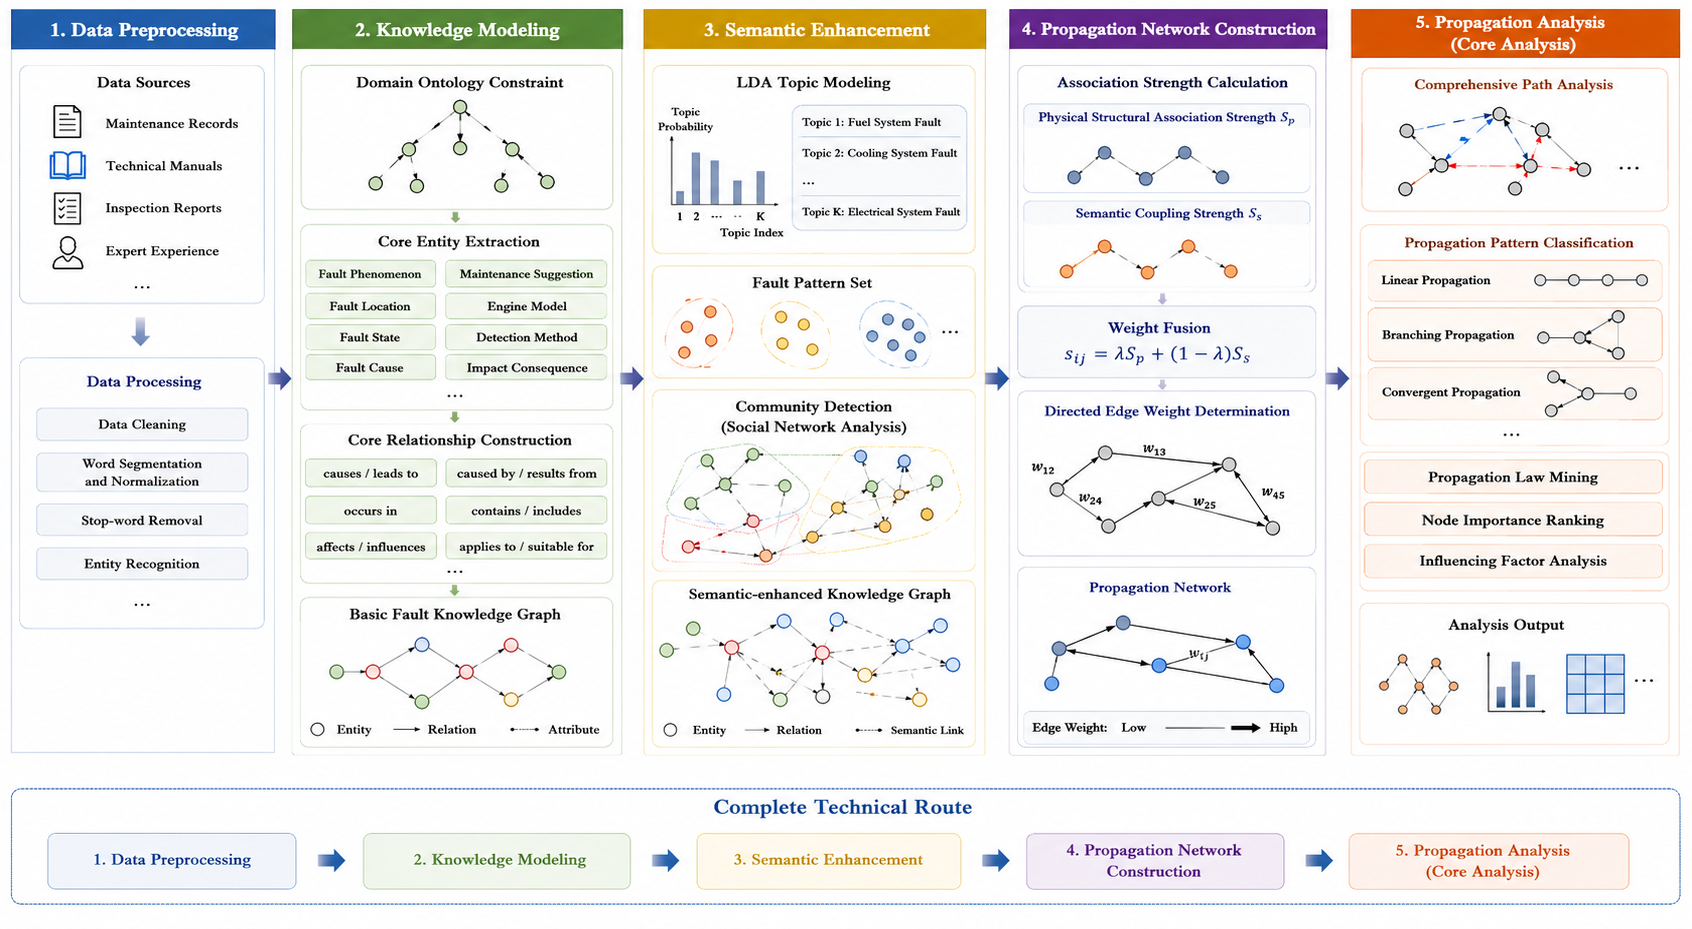
\includegraphics[width=.94\linewidth]{figures/framework.png}
\caption{Overall framework for semantic representation and candidate fault propagation analysis.}\label{fig:flowchart}
\end{figure}
\section{Construction of Semantic-Enhanced Network}
\subsection{Construction of Basic Fault Knowledge Graph}
The basic fault knowledge graph serves as the structural carrier for fault propagation analysis. Its core function is to establish structured associations among fault-related entities, providing a unified framework for the extraction and reasoning of propagation paths. Based on the engineering logic of diesel engine fault diagnosis, this paper constructs a domain ontology covering the entire life cycle of faults, and defines entity types, relationship types and attribute constraints to ensure the standardization and consistency of knowledge representation.
At the entity level, fault phenomena are regarded as observable external manifestations; fault locations correspond to physical structural carriers; fault states describe component failure modes; fault causes point to failure root causes; maintenance suggestions correspond to disposal strategies. Meanwhile, engine models, detection methods and impact consequences are incorporated to form a complete system of fault knowledge elements.

At the relationship level, causal candidates, structural membership, functional influence and spatial context are retained with distinct analysis roles. The structural experiments start from the saved Neo4j export supplied with the project. A separate updated-model pipeline performs new entity and ordered-pair relation inference over the complete corpus. Results from the saved graph and from fresh model predictions are reported with their respective inputs; structural measurements on the saved export are not presented as successful end-to-end extraction by the updated models.

The basic graph expresses explicit associations. Semantic augmentation adds topic attributes and rule-based mechanism abstractions to support traceable candidate reasoning. These abstractions are generated from disclosed mechanism matching and inherited input links; they are not independently observed intermediate failures.
\subsection{LDA-based Fault Semantic Topic Mining}
LDA models term co-occurrence to estimate latent topic distributions\cite{blei2003latent,roder2015exploring}. Figure~\ref{fig:LDA_Model} illustrates the generic modeling principle. In the executed corpus analysis, Jieba tokenization uses a fixed professional lexicon and $\mathrm{HMM}=\mathrm{false}$; terms must occur in at least two documents. The resulting vocabulary contains 1385 terms. The topic sweep uses seed 42, 20 passes, 200 iterations and candidate values $K=3,\ldots,12$.
The implemented coherence index is Gensim $c_v$, with ten topic words and a sliding window of 110. This choice is disclosed because the original manuscript does not specify the coherence variant. Figure~\ref{fig:LDA_Result} reports the executed sweep: the maximum is 0.3640 at $K=10$, whereas $K=7$ gives 0.3229. Seven topics are retained as a separately fixed configuration for structural analysis, rather than described as the measured optimum.
Keyword anchors map topic distributions onto seven engineering system labels: fuel and combustion, hydraulic, cooling and heat dissipation, electrical and control, mechanical wear and sealing, intake and exhaust, and transmission and steering. This mapping is a weak semantic attribution, not an independent physical-system annotation. The full-corpus topic sweep is descriptive; the grouped retrieval experiment fits its own fixed-$K=7$ topic model using training case bodies only.
\begin{figure}[tbp]
\centering
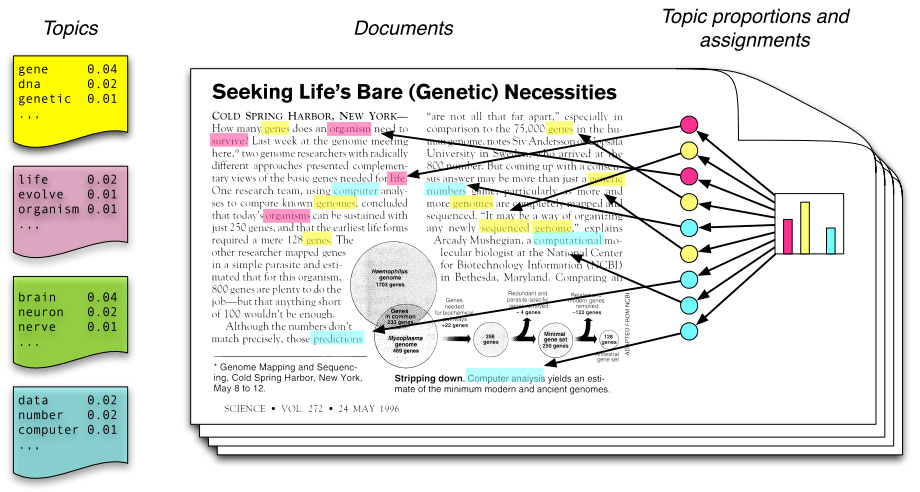
\includegraphics[width=.90\linewidth]{figures/lda_illustration.png}
\caption{Generic illustration of LDA topic modeling; the displayed example words are conceptual and are not diesel-corpus measurements.}\label{fig:LDA_Model}
\end{figure}
\begin{figure}[tbp]
\centering
\includegraphics[width=.92\linewidth]{figures/topic_coherence.pdf}
\caption{Executed full-corpus topic coherence sweep. The maximum is at ten topics; the seven-topic configuration is reported separately.}\label{fig:LDA_Result}
\end{figure}
\subsection{Fault Propagation Module Division Based on Community Analysis}
Based on semantic topics, the Louvain community detection algorithm is adopted to partition the modules of the fault propagation network. Following the criterion of modularity maximization, this algorithm iteratively optimizes the network partition structure through local node aggregation, enabling efficient mining of topological communities with high cohesion and low coupling in the network. Taking fault semantic correlation and propagation edge weights as the basis, the algorithm automatically identifies the aggregation characteristics and hierarchical boundaries of fault nodes. Its core objective is to detect fault semantic communities with high internal cohesion and low coupling, and reveal the aggregation attributes and hierarchical boundaries of fault propagation\cite{zhang2012journal}.

The enhanced saved graph has 224 automatic Louvain communities on its positive-weight undirected projection, with modularity 0.8877. Reciprocal directed weights are summed for this projection, and 442 isolated nodes are excluded from community assignment. These automatic communities are distinct from the seven keyword-anchored system labels. Figure~\ref{fig:Analyze_Hot} shows the directional association matrix under the weak system mapping; Fig.~\ref{fig:Analyze} reports the actual directed-pair weight distributions. The 2009 within-community pairs have a mean weight of 0.7120, compared with 0.5547 for 142 between-community pairs. These are structural association measurements and do not measure propagation speed, resistance or physical probability.
\begin{figure}[tbp]
\centering
\includegraphics[width=.87\linewidth]{figures/system_coupling.pdf}
\caption{Directional association mass under the weak seven-system mapping, normalized by the largest matrix entry. System labels are not independently reviewed physical annotations.}\label{fig:Analyze_Hot}
\end{figure}
\begin{figure}[tbp]
\centering
\includegraphics[width=.92\linewidth]{figures/community_weights.pdf}
\caption{Measured association-weight distributions within and between automatic Louvain communities of the enhanced saved graph.}\label{fig:Analyze}
\end{figure}
\subsection{Construction of Semantic-Enhanced Knowledge Graph}
The semantic-enhanced graph combines the saved entity/relationship structure with topic attributes and mechanism abstractions\cite{paulheim2016knowledge,chen2024information}. This extends the available representation with semantic and topological attributes while retaining traceable input links\cite{paul2019compact}. Figure~\ref{fig:KG} illustrates one case-specific graph before and after augmentation; the complete saved graph grows from 2063 nodes and 3156 typed edges to 2078 nodes and 3717 typed edges.
Node enhancement adds 15 mechanism classes and attaches topic distributions and weak system labels to existing entities. The 561 added typed edges express mechanism membership or inherited candidate associations. Their rule-derived status remains explicit. Louvain community identifiers describe a separate topological partition and are not equated with anatomical subsystem identities.
For an analysis edge $u\to v$, the association weight is
\begin{equation}
w_{uv}=\frac{S_{uv}+C_{uv}+P_{uv}}{3},\quad
S_{uv}=\frac{\theta_u^{\mathsf T}\theta_v}{\|\theta_u\|\|\theta_v\|},\quad
C_{uv}=\frac{|A_u\cap A_v|}{\sqrt{|A_u||A_v|}}.
\label{eq:association_weight}
\end{equation}
Here $\theta$ is the mean supported-case topic vector, $A$ is the case support set, and zero denominators give a zero similarity or co-occurrence value. $P_{uv}$ is a binary indicator of an explicit supporting input relation, not measured physical coupling strength. Parallel typed analysis edges are averaged into a directed pair. In the train-only ablation, $A$ contains distinct training case-body groups; in the descriptive saved-graph analysis it contains numbered case records. Equal coefficients and mechanism rules are disclosed completion assumptions. The resulting weights are uncalibrated association scores.
\begin{figure}[tbp]
\centering
\includegraphics[width=.98\linewidth]{figures/case_graph.pdf}
\caption{Saved graph for case 1 before and after mechanism augmentation. N11: turbocharger; N9: oil-seal aging and oil leakage; N7: low power under load and blue exhaust smoke; N10: oil-seal replacement; N4: restored power and normal exhaust. N3/N6/N8/N12/N13 are related aging/leakage mentions, and N5 is leakage. M1: aging mechanism; M2: leakage mechanism. The N10--N4 repair/recovery branch is context, not fault propagation.}\label{fig:KG}
\end{figure}
\section{Fault Propagation Paths and Pattern Analysis}
\subsection{Global Mining of Fault Propagation Paths}
All simple directed paths with at least two nodes are enumerated within case-supported subgraphs; the path nodes must share a supporting case record. All 1522 case computations complete without a hop cap. Unique ordered node sequences are counted separately from path--case incidences. The saved base graph yields 2084 unique context paths and 6241 incidences; the augmented graph yields 4506 paths and 14699 incidences. Literal support denotes co-mention in a retrospective text and does not establish an observed causal sequence.
A second screen requires an endpoint representing a fault phenomenon or consequence, at least one causal, functional-influence or inherited mechanism candidate edge, and restricted positions for structural and manifestation context. Membership-only paths and redundant literal-member/mechanism-class combinations are excluded. This gives 1043 qualified candidates before augmentation and 1338 afterward; 359 and 526 respectively contain at least three nodes. The increase is a structural candidate-count result, not a path-completeness rate against independently annotated true chains.
Table~\ref{tab:ClassicFaultChain} lists selected candidate chains with fault endpoints, including fuel-filter water accumulation and thermostat sticking. Frequencies count supporting numbered records and distinct case bodies separately. The mean path weight is the arithmetic mean of directed association weights. These examples require engineering review before use as confirmed propagation chains; candidates involving recovery language or ambiguous direction remain an adjudication concern.
\begin{table}[tbp]
\centering
\paperTableStyle
\caption{Selected candidate chains from the saved graph.}\label{tab:ClassicFaultChain}
\begin{tabular*}{\linewidth}{@{\extracolsep{\fill}}P{.59\linewidth}L{.10\linewidth}L{.09\linewidth}L{.14\linewidth}@{}}
\toprule
\textbf{Candidate chain} & \textbf{Records} & \textbf{Bodies} & \textbf{Mean weight} \\
\midrule
Fuel filter $\to$ Water accumulation\newline $\to$ Engine vibration & 15 & 7 & 0.8667 \\
\addlinespace[3pt]
Thermostat $\to$ Thermostat sticking\newline $\to$ Engine overheating & 11 & 7 & 0.9547 \\
\addlinespace[3pt]
Thermostat $\to$ Stuck-closed thermostat\newline $\to$ Engine overheating & 10 & 6 & 0.9396 \\
\addlinespace[3pt]
Alternator belt $\to$ Belt breakage\newline $\to$ No alternator output & 8 & 4 & 1.0000 \\
\addlinespace[3pt]
Fuel tank $\to$ Water at tank bottom\newline $\to$ Engine vibration & 8 & 4 & 0.9440 \\
\bottomrule
\end{tabular*}
\paperTableNote{Numbered records and distinct case bodies are reported separately; weights are association scores.}
\end{table}

\subsection{Classification and Characteristic Analysis of Typical Fault Propagation Modes}
A linear topology candidate is a complete weak component consisting of a directed chain of at least three nodes, without branching, convergence or cycles\cite{buldyrev2010catastrophic,gan2020prognostics}. Under case-supported causal/functional/inherited projections, the base graph has 60 unique linear sequences and 126 case incidences. After augmentation these become 20 sequences and 42 incidences. Added mechanism connections can convert a previously linear component into another topology, so pattern counts need not increase monotonically.
A branching candidate comprises one source and a pair of immediate downstream nodes that are mutually unreachable\cite{xing2008fault,loria2018strict,liu2020robust}. The base and augmented graphs contain 94 and 131 unique branching candidates, with 208 and 282 case incidences respectively. This is a static one-to-many relation pattern; it does not establish simultaneous failure, faster diffusion or a higher hazard level.
A convergent candidate comprises a shared target and two mutually unreachable immediate predecessor nodes\cite{li2021energy}. The corresponding counts increase from 126 to 319 unique candidates, and from 341 to 836 case incidences. Topological separation is not proof that the sources are physically independent. These counts therefore characterize static graph motifs rather than observed multi-fault superposition.
\section{Structural Characteristics of Candidate Propagation}
Figure~\ref{fig:law}(a) summarizes case-supported linear, branching and convergent topology counts. The higher mean association weight within automatic communities is consistent with semantic and co-occurrence clustering in this graph. Because the same features contribute to graph construction, the within/between difference is descriptive evidence rather than independent validation of physical transmission. It can guide candidate prioritization, but its effect on practical troubleshooting requires external assessment.

Figure~\ref{fig:law}(b) reports each weakly mapped system's incident cross-system weight as a share of twice the total mapped cross-system directed weight. In this execution, mechanical wear and sealing ranks first with 26.09\%, followed by transmission and steering at 21.14\% and hydraulics at 20.92\%; fuel and combustion accounts for 3.05\%. These outcomes depend on the saved graph, corpus composition and weak mapping. They do not support a general claim that fuel injection and combustion is the dominant physical fault-transmission hub, nor do centrality measures constitute hub-identification accuracy.

The qualified augmented paths are also classified by static scope, as shown in Fig.~\ref{fig:law}(c): 281 component-level, 191 subsystem-level, 534 cross-system candidates, four with explicit engine-consequence terms, and 328 with unknown scope. A cross-system path is not automatically a whole-engine failure. Without equipment/event identifiers and timestamps, these scope categories cannot establish a chronological three-stage evolution, propagation velocity or severity escalation. They provide hypotheses for subsequent event-based validation.
\begin{figure}[tbp]
\centering
\includegraphics[width=.97\linewidth]{figures/static_structure.pdf}
\caption{Computed static graph characteristics: (a) case-supported topology counts; (b) incident cross-system weight shares under weak system mapping; (c) qualified candidate-path scope. No temporal or severity observations are plotted.}\label{fig:law}
\end{figure}
\section{Computational Evaluation and Validation Scope}
The evaluation separates supplied-label extraction benchmarks, full-corpus candidate inference, saved-graph structural analysis and grouped silver-reference retrieval. The aligned NER encoder uses the BERT-compatible architecture of the supplied pretrained checkpoint, instead of the source RoBERTa constructor. NER training uses maximum sequence length 512, batch size eight, learning rate $2\times10^{-5}$, dropout 0.2, weight decay 0.01, and a maximum of 15 epochs with seed 42. Relation-model training uses maximum sequence length 128, batch size 32, learning rate $10^{-5}$, dropout 0.2, weight decay $10^{-4}$, AdamW and the original cosine warm-restart scheduler. Both training variants use development-set checkpoint selection; the reported NER metric requires exact span boundaries and entity type. Table~\ref{tab:ner_metrics} shows that the aligned model obtains 81.31\% F1 overall, 96.04\% on the template subset, and 5.24\% on the 90-record case-text subset. Reporting only the aggregate would conceal this distribution gap.

An exploratory adaptation freezes the encoder and trains the classifier using a fixed 60/15/15 partition of the 90 case-text records. Development selection equally weights template and case-text F1. On the same final 15 records, F1 changes from 6.98\% to 26.92\%. These records had been inspected previously and overlap the analysis corpus, so this is an internal adaptation diagnostic, not a newly independent industrial test.
\begin{table}[tbp]
\centering
\paperTableStyle
\caption{NER results using exact span and entity type matching.}\label{tab:ner_metrics}
\begin{tabular*}{\linewidth}{@{\extracolsep{\fill}}L{.20\linewidth}L{.285\linewidth}L{.175\linewidth}L{.145\linewidth}L{.126\linewidth}@{}}
\toprule
\textbf{Model} & \textbf{Evaluation subset} & \textbf{Precision~(\%)} & \textbf{Recall~(\%)} & \textbf{F1~(\%)} \\
\midrule
Source loading & Mixed test (890) & 50.80 & 77.15 & 61.26 \\
 & Template subset (800) & 68.92 & 83.65 & 75.57 \\
 & Case-text subset (90) & 0.83 & 4.09 & 1.37 \\
\midrule
Aligned encoder & Mixed test (890) & 73.94 & 90.32 & 81.31 \\
 & Template subset (800) & 94.78 & 97.33 & 96.04 \\
 & Case-text subset (90) & 3.39 & 11.55 & 5.24 \\
\midrule
Before adaptation & Internal case test (15) & 4.64 & 14.14 & 6.98 \\
After adaptation & Internal case test (15) & 19.72 & 42.42 & 26.92 \\
\bottomrule
\end{tabular*}
\paperTableNote{Precision, recall and F1 are percentages. The final two rows use a separate exploratory internal partition.}
\end{table}

The relation model is selected at epoch 14 using development accuracy, with seed 42 and 15 completed epochs. Inferred subject/object template groups are separated, and entity offsets are supplied by the benchmark. Of 348 heldout examples, 202 are classified correctly: accuracy is 58.05\% and nine-class macro F1 is 55.00\% (Table~\ref{tab:re_metrics}). The original 225-example test gives 61.33\% accuracy and 60.82\% macro F1 but had been evaluated historically. Both benchmarks contain nine positive relation classes and no reviewed no-relation class; they evaluate forced-choice classification rather than relation existence, pair precision or root-cause diagnosis.
\begin{table}[tbp]
\centering
\paperTableStyle
\caption{Positive-only relation classification.}\label{tab:re_metrics}
\begin{tabular*}{\linewidth}{@{\extracolsep{\fill}}L{.43\linewidth}L{.13\linewidth}L{.18\linewidth}L{.18\linewidth}@{}}
\toprule
\textbf{Benchmark} & \textbf{Examples} & \textbf{Accuracy~(\%)} & \textbf{Macro~F1~(\%)} \\
\midrule
Inferred-template heldout & 348 & 58.05 & 55.00 \\
Previously evaluated original test & 225 & 61.33 & 60.82 \\
\bottomrule
\end{tabular*}
\paperTableNote{These results do not evaluate relation existence or end-to-end root-cause diagnosis.}
\end{table}

The updated NER and grouped relation checkpoints are applied to all 1522 cases, producing 18704 entity mentions and 238728 ordered occurrence-pair predictions. Table~\ref{tab:thresholds} reports sensitivity to an added, uncalibrated confidence gate. At threshold 0.8 no candidate observations survive. Disabling that gate while retaining minimum entity length two and type constraints yields 14348 observations across 1480 cases and 10147 canonical typed edges. Of these observations, 12447 are maintenance-recommendation relations. Threshold zero is a disclosed diagnostic configuration, not a calibrated operating point or evidence of causal precision.
\begin{table}[tbp]
\centering
\paperTableStyle
\caption{Sensitivity of the updated-model candidate extraction to an uncalibrated confidence threshold.}\label{tab:thresholds}
\begin{tabular*}{\linewidth}{@{\extracolsep{\fill}}L{.16\linewidth}L{.24\linewidth}L{.21\linewidth}L{.31\linewidth}@{}}
\toprule
\textbf{Threshold} & \textbf{Observations} & \textbf{Cases} & \textbf{Typed edges} \\
\midrule
0.0 & 14,348 & 1,480 & 10,147 \\
0.2 & 10,807 & 1,373 & 7,406 \\
0.4 & 77 & 36 & 51 \\
0.6 & 0 & 0 & 0 \\
0.8 & 0 & 0 & 0 \\
\bottomrule
\end{tabular*}
\paperTableNote{Threshold zero disables the confidence gate; the length and entity-type gates remain active.}
\end{table}

Ten train-only graph variants combine five weight modes (unweighted, semantic, co-occurrence, physical-support proxy and equal fusion) with mechanism augmentation enabled or disabled. Normalized-body groups are kept together: 1071/226/225 numbered records correspond to 949/205/206 unique training/development/test groups. Topic and graph co-occurrence statistics are fitted using training groups only, with $K=7$ fixed in advance. Independence of the supervised extraction training sources from all corpus groups is not established.

For the updated-model train graph, augmentation changes the node count from 3668 to 3683 and typed analysis-edge count from 467 to 682. Weight-only modes preserve adjacency. The binary physical-support feature equals one for every retained analysis edge, so its ablation coincides with the unweighted graph. A separate comparison applies both model families to the same 69 frozen model-derived reference groups (Table~\ref{tab:silver}). The frozen unweighted and fused graphs each obtain 5.07\% Recall@3; their MRR values are 0.0859 and 0.0797. The updated-model variants obtain zero on these same reference metrics. These results do not establish improved retrieval or diagnostic accuracy. The reference set is based on the frozen models and favors their label space; it is not human-confirmed root-cause ground truth.
\begin{table}[tbp]
\centering
\paperTableStyle
\caption{Retrieval against the same 69 frozen model-derived reference groups.}\label{tab:silver}
\begin{tabular*}{\linewidth}{@{\extracolsep{\fill}}L{.22\linewidth}L{.34\linewidth}L{.21\linewidth}L{.15\linewidth}@{}}
\toprule
\textbf{Models} & \textbf{Graph variant} & \textbf{Recall@3~(\%)} & \textbf{MRR} \\
\midrule
Frozen models & Unweighted & 5.07 & 0.0859 \\
 & Fusion + mechanisms & 5.07 & 0.0797 \\
\midrule
Updated models & Unweighted & 0.00 & 0.0000 \\
 & Fusion + mechanisms & 0.00 & 0.0000 \\
\bottomrule
\end{tabular*}
\paperTableNote{Recall@3 is a percentage; MRR is unitless. These references are silver labels and favor the frozen-model label space.}
\end{table}


A future expert evaluation may use the proposed semantic interpretability score (SIS) in Eq.~\ref{eq:interpretability_score}, with the rubric in Table~\ref{tab:interpretability_metrics}. The four components are semantic coverage, path completeness, coupling clarity and diagnostic accuracy. No real per-rater scoring records are available in this experiment, so neither an observed SIS value nor an improvement in expert-assessed interpretability is reported. Structural coverage and path counts are not substituted for these expert ratings.
\begin{equation}
S_{\text{IS}} = 0.3 S_{\text{SC}} + 0.25 S_{\text{PC}} + 0.25 S_{\text{CC}}
+  0.2 S_{\text{DA}}
\label{eq:interpretability_score}
\end{equation}
\begin{table}[tbp]
\centering
\paperTableStyle
\fontsize{10.5}{13}\selectfont
\caption{Proposed expert interpretability rubric for future independent evaluation.}\label{tab:interpretability_metrics}
\begin{tabular*}{\linewidth}{@{\extracolsep{\fill}}P{.19\linewidth}P{.365\linewidth}P{.405\linewidth}@{}}
\toprule
\textbf{Sub-index} & \textbf{Description and definition} & \textbf{Scoring logic (0--10)} \\
\midrule
$S_{\text{SC}}$\newline (Semantic Coverage) & Coverage of fault mechanisms by semantic nodes. Measures the completeness of semantic nodes covering key diesel engine fault mechanisms & \textbf{9--10 pts:} covers all core failure links (fuel supply, combustion, cooling, etc.);\newline \textbf{5--8 pts:} covers partial key links;\newline \textbf{$<$5 pts:} lacks valid semantic nodes \\
\addlinespace[5pt]
$S_{\text{PC}}$\newline (Path Completeness) & Integrity of failure chains. Measures whether causal paths from physical failure to semantic propagation to fault consequences are complete & \textbf{9--10 pts:} fully covers ``physical failure $\to$ semantic propagation $\to$ fault consequence'';\newline \textbf{5--8 pts:} missing partial propagation links;\newline \textbf{$<$5 pts:} only physical-level connections exist \\
\addlinespace[5pt]
$S_{\text{CC}}$\newline (Coupling Clarity) & Clarity of cross-system semantic coupling. Measures the clarity and traceability of causal coupling relationships between subsystems & \textbf{9--10 pts:} all cross-system coupling paths (e.g., temp. change $\to$ combustion anomaly) clearly marked;\newline \textbf{5--8 pts:} partial coupling paths missing;\newline \textbf{$<$5 pts:} no cross-system coupling marked \\
\addlinespace[5pt]
$S_{\text{DA}}$\newline (Diagnostic Accuracy) & Support capability for fault diagnosis. Measures the support of the knowledge graph for root cause localization and fault evolution prediction in practical diagnosis & \textbf{9--10 pts:} accurately locates root causes and predicts fault diffusion trends;\newline \textbf{5--8 pts:} locates failure links but cannot predict evolution;\newline \textbf{$<$5 pts:} only displays physical connections \\
\bottomrule
\end{tabular*}
\paperTableNote{No observed scores are available.}
\end{table}
Figure~\ref{fig:compare} reports the measured size of the saved graph and its qualified candidate-path counts. These measurements demonstrate the effect of semantic augmentation on representation and candidate enumeration. Independent root-cause and complete-path annotations are still required for diagnostic accuracy or path-completeness rates. No engineer localization times, independent quantitative physical association strengths or timestamped propagation events are available; therefore efficiency improvements and dynamic evolutionary claims are not evaluated.
\begin{figure}[tbp]
\centering
\includegraphics[width=.96\linewidth]{figures/structural_comparison.pdf}
\caption{Measured saved-graph node and typed-edge counts and qualified candidate-path counts before and after augmentation. These counts are not diagnostic accuracy or expert SIS.}\label{fig:compare}
\end{figure}
\section{Discussion}
The executed framework makes ontology attributes, topic distributions, case support, mechanism rules and candidate paths inspectable. Its demonstrated benefit is an expanded, traceable representation for retrospective maintenance-text analysis. Structural augmentation and path enumeration are measurable outcomes, whereas improved diagnostic accuracy and expert interpretability require separate evidence.

Semantic association is stronger within the automatic communities in this execution, but the communities are partly defined by those same weights. The seven engineering labels are a weak keyword/topic mapping, and the automatic partition contains 224 communities. Mechanical wear and sealing carries the largest mapped incident cross-system weight. Consequently neither a seven-community physical decomposition nor fuel-system dominance is established as an invariant of diesel-engine fault propagation.

The extraction benchmarks show a substantial distribution gap. High F1 on recurring template-style sentences does not carry over to the case-text subset. Internal classifier adaptation improves the disclosed 15-record result but remains small and retrospective. Positive-only relationship classification also leaves relation existence unresolved. The empty candidate output at threshold 0.8 and the low silver-reference retrieval scores make extraction quality and confidence calibration central priorities for further work.

Linear, branching, convergent and multi-scope structures describe static candidate topology. Mechanism bridges may increase branching and convergence while reducing the number of purely linear components. Neither this topology nor the number of candidate paths proves chronological fault evolution, simultaneous failures, completeness of true causal chains or severity escalation. Event-based validation is needed before converting these structures into operational warning thresholds.

The principal limitations are incomplete case-source provenance, duplicate and recurring template structure, weak system mapping, a binary rather than measured physical association feature, absence of no-relation annotations, and lack of independently reviewed root causes and complete paths. Real expert SIS ratings and engineer fault-localization timing records are also missing. The computational results reported here exclude the separately labeled simulated validation workbook; simulation is not used as industrial validation evidence.

Future research can be conducted in several directions. First, multi-source heterogeneous industrial data such as sensor streams, vibration signals, maintenance logs, and operational records can be integrated to improve the real-time perception capability of the propagation network. Second, graph neural networks and large language models can be introduced to enhance semantic reasoning capability and adaptive propagation prediction performance. Third, temporal knowledge graph technology can be incorporated to model dynamic fault evolution processes under varying operating conditions. Finally, the proposed framework can be combined with digital twin systems to establish real-time fault propagation simulation and intelligent maintenance decision-making platforms for complex diesel engine systems.
\section{Conclusion}
This study implements a semantic-enhanced knowledge graph framework for retrospective diesel-engine maintenance case analysis. The 1522 numbered records comprise 1360 normalized case bodies. Under the disclosed full-corpus settings, LDA coherence is highest at ten topics ($c_v=0.3640$); the seven-topic configuration is retained as a separate fixed structural analysis. Augmentation of the saved graph adds 15 mechanism classes and 561 typed edges, and raises the number of rule-qualified candidate paths from 1043 to 1338. Automatic communities, case-supported motifs and static scope classes provide inspectable descriptions of the resulting association network.

The measured extraction results limit the supported claims: aligned NER F1 is 81.31\% on the mixed benchmark and 5.24\% on its case-text subset, while positive-only relation classification reaches 58.05\% accuracy and 55.00\% macro F1 on inferred-template-heldout examples. Internal adaptation and grouped graph experiments are reported with their evaluation boundaries. The frozen-reference comparison does not demonstrate a retrieval improvement for the updated models. These results support an executable computational framework and identify unresolved extraction and validation requirements. Future work should obtain independently reviewed relation-existence and causal-path annotations, quantitative physical labels, expert scores, engineer timing records and timestamped equipment events before claiming diagnostic gains or temporal fault evolution.
\begin{acknowledgments}
This work was supported by the Open Fund of National Key Laboratory of Internal Combustion Engine and Power Systems (Grant No. skleps-sq-2024-170).
\end{acknowledgments}

\bibliographystyle{maik}
\bibliography{ref}
\end{document}
